%%%%%%%%%%%%%%%%%%%%%%%%%
% Dokumentinformationen %
%%%%%%%%%%%%%%%%%%%%%%%%%
\newcommand{\titleinfo}{Elektronik 1 - Formelsammlung}
\newcommand{\authorinfo}{Braun \& Co, J. Rast}
\newcommand{\versioninfo}{$Revision: 0 $ - powered by \LaTeX} 
%
%%%%%%%%%%%%%%%%%%%%%%%%%%%%%%%%%%%%%%%%%%%%%
% Standard projektübergreifender Header für
% - Makros 
% - Farben
% - Mathematische Operatoren
%
% DORT NUR ERGÄNZEN, NICHTS LÖSCHEN
%%%%%%%%%%%%%%%%%%%%%%%%%%%%%%%%%%%%%%%%%%%%%
% Genereller Header
\documentclass[10pt,twoside,a4paper,fleqn]{article}
\usepackage[utf8]{inputenc}
\usepackage[left=1cm,right=1cm,top=1cm,bottom=1cm,includeheadfoot]{geometry}
\usepackage[ngerman]{babel,varioref}

% Pakete
\usepackage{amssymb,amsmath,fancybox,graphicx,color,lastpage,wrapfig,fancyhdr,hyperref,verbatim}

%%%%%%%%%%%%%%%%%%%%
% Generelle Makros %
%%%%%%%%%%%%%%%%%%%%
\newcommand{\formelbuch}[1]{$_{\textcolor{red}{\mbox{\small{S#1}}}}$}
\newcommand{\verweis}[2]{\small{(siehe auch \ref{#1}, #2 (S. \pageref{#1}))}}
\newcommand{\subsubadd}[1]{\textcolor{black}{\mbox{#1}}}


\newcommand{\skriptsection}[2]{\section{#1 {\tiny Skript S. #2}}}
\newcommand{\skriptsubsection}[2]{\subsection{#1 {\tiny Skript S. #2}}}
\newcommand{\skriptsubsubsection}[2]{\subsubsection{#1 {\tiny Skript S. #2}}}

%%%%%%%%%%
% Farben %
%%%%%%%%%%
\definecolor{black}{rgb}{0,0,0}
\definecolor{red}{rgb}{1,0,0}
\definecolor{white}{rgb}{1,1,1}
\definecolor{grey}{rgb}{0.8,0.8,0.8}

%%%%%%%%%%%%%%%%%%%%%%%%%%%%
% Mathematische Operatoren %
%%%%%%%%%%%%%%%%%%%%%%%%%%%%
\DeclareMathOperator{\sinc}{sinc}



% Fouriertransformationen
\unitlength1cm
\newcommand{\FT}
{
\begin{picture}(1,0.5)
\put(0.2,0.1){\circle{0.14}}\put(0.27,0.1){\line(1,0){0.5}}\put(0.77,0.1){\circle*{0.14}}
\end{picture}
}


\newcommand{\IFT}
{
\begin{picture}(1,0.5)
\put(0.2,0.1){\circle*{0.14}}\put(0.27,0.1){\line(1,0){0.45}}\put(0.77,0.1){\circle{0.14}}
\end{picture}
}



%%%%%%%%%%%%%%%%%%%%%%%%%%%%
% Allgemeine Einstellungen %
%%%%%%%%%%%%%%%%%%%%%%%%%%%%
%pdf info
\hypersetup{pdfauthor={\authorinfo},pdftitle={\titleinfo},colorlinks=false}
\author{\authorinfo}
\title{\titleinfo}

%Kopf- und Fusszeile
\pagestyle{fancy}
\fancyhf{}
%Linien oben und unten
\renewcommand{\headrulewidth}{0.5pt} 
\renewcommand{\footrulewidth}{0.5pt}

\fancyhead[L]{\titleinfo{ }\tiny{(\versioninfo)}}
%Kopfzeile rechts bzw. aussen
\fancyhead[R]{Seite \thepage { }von \pageref{LastPage}}
%Fusszeile links bzw. innen
\fancyfoot[L]{\footnotesize{\authorinfo}}
%Fusszeile rechts bzw. ausen
\fancyfoot[R]{\footnotesize{\today}}

% Einrücken verhindern versuchen
\setlength{\parindent}{0pt}



% Möglichst keine Ergänzungen hier, sondern in header.tex
\begin{document}

	\section{Grundbegriffe \formelbuch{1}}
	
		\subsection{DC- und Kleinsignal-Ersatzschaltung \formelbuch{1-15}}
			\begin{minipage}{18cm}
            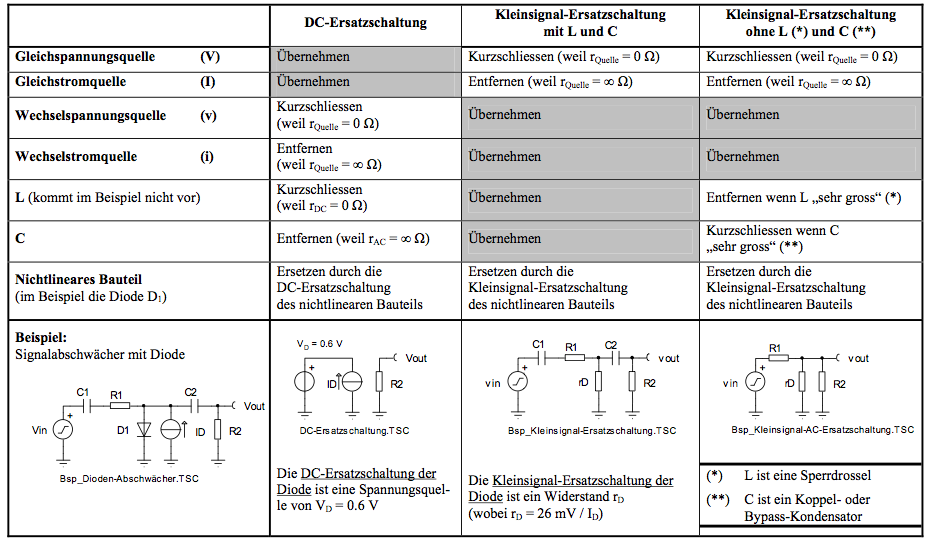
\includegraphics[width=18cm]{./bilder/dc-kleinsignal-ersatz.png}
            \end{minipage}

		\subsection{Verstärkertypen \formelbuch{1-26}}
			\begin{minipage}{10cm}
            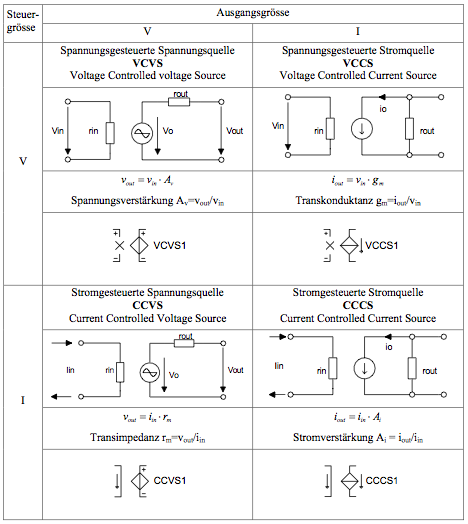
\includegraphics[width=10cm]{./bilder/verstaerkertypen.png}
            \end{minipage}
			\begin{minipage}{8cm}
            {\bf Verstärkerfaktoren:}\\
            - Spannungs-Verstärkerfaktor \hspace{4mm}$A_v$ (ohne Einheit)\\
            - Strom-Verstärkungsfaktor \hspace{6mm} $A_i$ (ohne Einheit)\\
            - Transkonduktanz \hspace{19mm} $g_m$ (Einheit $\Omega^{-1}$)\\
            - Transresistanz \hspace{24mm} $r_m$ (Einheit $\Omega$)\\ \\
            Dynam. Eingangswiderstand \hspace{5mm} $r_{in}$ ($\Omega$)\\
            Dynam. Ausgangswiderstand \hspace{4mm} $r_{out}$ ($\Omega$)\\ \\
            {\bf Bei idealen gesteuerten Quellen gelten folgende Werte für
            $r_{in}$ und $r_{out}$:}\\
            Bei Stromsteuerung ist \hspace{13.5mm} $r_{in}=0 \Omega$\\
            Bei Spannungssteuerung ist \hspace{6.5mm} $r_{in}=\infty \Omega$\\
            Beim Stromausgang ist \hspace{13.5mm} $r_{out}=\infty \Omega$\\
            Beim Spannungsausgang ist \hspace{6.5mm} $r_{out}=0 \Omega$\\
            
            {\bf Invertierender Verstärker:}\\
            Verstarkungsfaktor ist negativ $(A<0)$\\
            $v_{out}$ verläuft {\it gegenphasig} zu $v_{in}$\\
            
            {\bf Nichtinvertierender Verstärker:}\\
            Verstärkungsfaktor ist positiv $(A>0)$\\
            $v_{out}$ verläuft {\it gleichphasig} zu $v_{in}$
            \end{minipage}
	
	
		\subsection{Dezibel (dB) \formelbuch{1-25}}
			\begin{tabular}{p{10cm}p{8cm}}
        		Das Dezibel der Verhältniszahl $V$ wird wie folgt berechnet:
        		& \fbox{$V_{dB}=20 log \left| V\right|$}\\
        		Aus der gegebenen Dezibel-Zahl $V_{dB}\to$ lineare Verhältniszahl:
        		& \fbox{$V=10^{\frac{V_{dB}}{20dB}}$}\\ \\
        \end{tabular}

\hrule

		\subsection{Übertragungsfaktoren \formelbuch{1-24}}
			\begin{minipage}{18cm}
	   	    	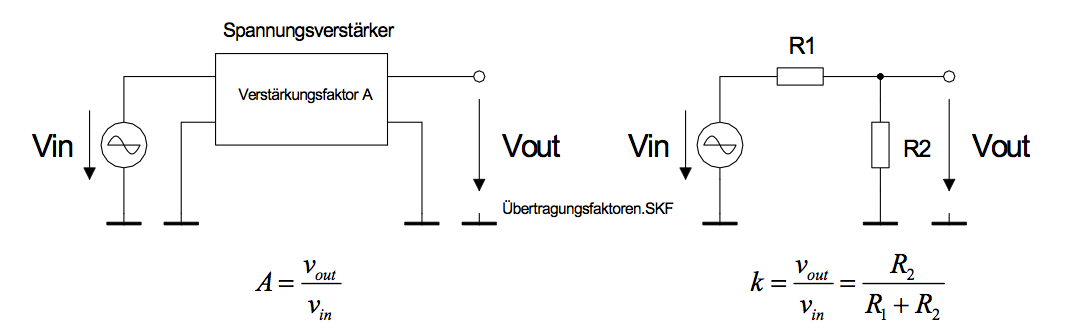
\includegraphics[width=16cm]{./bilder/uebertragungsfaktoren.png}
       		\end{minipage}

\hrule

		\subsection{Grosssignalwiderstand \formelbuch{1-11}}
			Gleichstromwiderstand $R$ \hspace{15mm} $R=\frac{V_R}{I_R}$
			$\left(\frac{\mbox{Gleichspannung im Arbeitspunkt}}{\mbox{Gleichstrom im
			Arbeitspunkt}}\right)$\\ \\
			Bei {\it linearen Widerständen} hängt der Grosssignalwiderstand
			{\it nicht} vom Arbeitspunkt ab.\\
			Bei {\it nicht linearen Widerständen} hängt der Grosssignalwiderstand
			vom Arbeitspunkt ab. $\Rightarrow$ Interessiert aber in der Elektronik nicht.
			Sind immer am Kleinsignalwiderstand $r$ intressiert.\\
		
\hrule
		
		\subsection{Kleinsignalwiderstand (dynamischer oder differenzieller
		Widerstand) \formelbuch{1-13}}
			Kleinsignalwiderstand $r$ \hspace{15mm} $r_L=\frac{dV_L}{dI_L}$ In der Praxis
			verwenden wir die Näherung $r_L=\frac{dV_L}{dI_L}\approx \frac{\Delta
			V_L}{\Delta I_L}$\\ \\
			Wenn die Strom-Spannungskennlinie $V=f(I)$ mathematisch gegeben ist, erhalten
			wir den Kleinsignalwiderstand $r_L$ durch Differenzierung der
			Kennliniengleichung $V_L=f(I_L)$ im Arbeitspunkt $(I_L, V_L)$.\\
			Bei {\it nichtlinearen Zweipolen} hängt der Kleinsignalwiderstand $r$
			vom Arbeitspunkt ab, aber $r\neq R$\\
			Bei {\it linearen Zweipolen} ist der Kleinsignalwiderstand $r$
			identisch mit dem DC-Widerstand $R$. Desshalb ist $r$ bei {\it linearen
			Zweipolen} vom Arbeitspunkt {\it unabhängig}.\\
		
\hrule
		
		\subsection{Überlagerungssatz für lineare Systeme \formelbuch{1-14}}
			Wenn das Eingangssignal eines linearen Verstärkers (oder allgemein eines
			linearen Netzwerkes) aus einer Summe von zwei verschiedenen Signalen besteht,
			dürfen wir die beiden Teilsignale getrennt mit dem Verstärkungsfaktor
			multiplizieren und die beiden resultierenden Ausgangssignale am Ausgang
			addieren.\\
			\hspace*{10mm}
			\fbox{$v_{out \hspace{1mm}
			total}=(v_{in1}+v_{in2})A=v_{in1}A+v_{in2}A=v_{out1}+v_{out2}=v_{in
			\hspace{1mm}total}A$}\\
	
% \newpage
% 	\section{Dioden \formelbuch{2}}
% 	\subsection{Diodenarten \formelbuch{2-3}}
% 	\subsection{Varaktordiode \formelbuch{2-4}}
% 	\subsection{LED und Laserdiode \formelbuch{2-5}}
% 	\subsection{Photodiode \formelbuch{2-5}}
% 	\subsection{Z-Diode \formelbuch{2-6}}
% 	
\newpage
	\section{Operationsverstärker \formelbuch{3}}
		\subsection{Opamp Schaltungen}
		\subsubsection{Invertierender Verstärker \formelbuch{3-7}}
			\begin{minipage}[T]{12cm}
          	  Bein invertierenden Verstärker ist die Ausgangsspannung gegenphasig
            	zur Eingangsspannung.\\
            	Closed-Loop Spannung:
            	\hspace{23mm}\fbox{$A_{CL}=\frac{v_{out}}{v_{in}}=-
            	\frac{R_F}{R_1}$}\\
            	\hspace*{10mm}\fbox{$i_1=\frac{v_{in}+v_d}{R_1}$}
           		\hspace{29.5mm}\fbox{$i_F=-\frac{v_{out}+v_d}{R_F}$}\\
            	Ausgangswiderstand des I-Verstärkers: \fbox{$r_{out}=0\Omega$}\\
            	Eingangswiderstand des I-Verstärkers:
            	\hspace{0.5mm}\fbox{$r_{in}=R_1$}
            \end{minipage}
			\begin{minipage}{6cm}
            	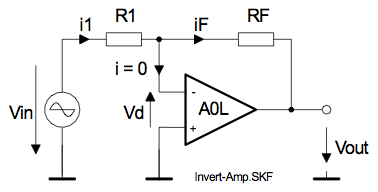
\includegraphics[width=6cm]{./bilder/i-verstaerker.png}
            \end{minipage}\\

\hrule

		\subsubsection{Nichtinvertierender Verstärker \formelbuch{3-10}}
			\begin{minipage}[T]{12cm}
            	Bein nichtinvertierenden Verstärker ist die Ausgangsspannung
            	gleichphasig zur Eingangsspannung.\\ Closed-Loop Gain:
            	\hspace{32mm}
            	\fbox{$A_{CL}=\frac{v_{out}}{v_{in}}=\frac{R_F}{R_1}+1$}\\
            	\hspace*{10mm}\fbox{$i_1=\frac{v_{in}-v_d}{R_1}$}
            	\hspace{32mm}\fbox{$i_F=\frac{v_{out}}{R_F+R_1}$}\\
            	Ausgangswiderstand des NI-Verstärkers: \fbox{$r_{out}=0\Omega$}\\
            	Eingangswiderstand des NI-Verstärkers:
            	\hspace{1mm}\fbox{$r_{in}=\infty$}
            \end{minipage}
			\begin{minipage}{6cm}
            	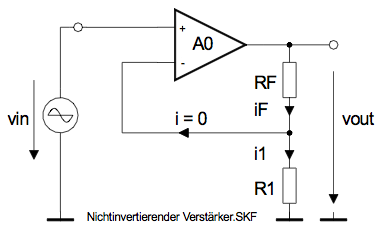
\includegraphics[width=6cm]{./bilder/ni-verstaerker.png}
            \end{minipage}\\

\hrule

		\subsubsection{Verstärker mit mehreren Eingängen \formelbuch{3-12}}
			\begin{minipage}{12.5cm}
            	\hspace*{10mm}\fbox{$A_{CL1}=-\frac{R_F}{R_1}$}
            	\hspace{15mm}\fbox{$A_{CL2}=-\frac{R_F}{R_2}$}\\
            	\hspace*{10mm}\fbox{$A_{CL3}=\frac{R_F+(R_1//R_2)}{(R_1//R_2)}$}\\
            	\hspace*{10mm}\fbox{$v_{out}=A_{CL1}v_1+A_{CL2}v_2+A_{CL3}v_3=
            	-\frac{R_F}{R_1}v_1-\frac{R_F}{R_2}v_2+\frac{R_F+(R_1//R_2)}{(R_1//R_2)}$}
            \end{minipage}
			\begin{minipage}{5.5cm}
            	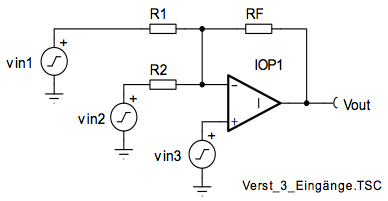
\includegraphics[width=5.5cm]{./bilder/3-eingaenge.png}
            \end{minipage}\\

\hrule

		\subsubsection{Invertierender Addierer \formelbuch{3-20}}
			\begin{minipage}[b]{12cm}
            \hspace*{10mm}\fbox{$V_{out}=A_{CL1}V_{IN1}+A_{CL2}V_{IN2}+\ldots$}\\
            \hspace*{10mm}\fbox{$A_{CL1}=- \frac{R_F}{R_1}$}
           	\hspace*{10mm}\fbox{$A_{CL2}=- \frac{R_F}{R_2}$}
            \end{minipage}
			\begin{minipage}{6cm}
            	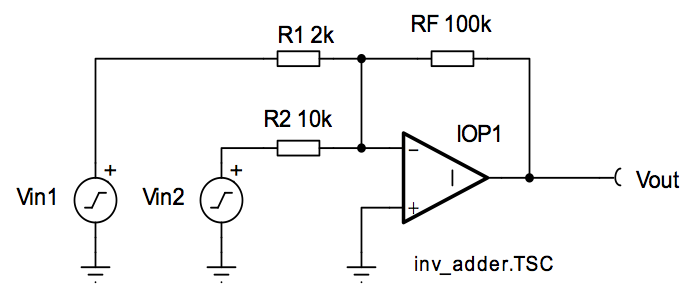
\includegraphics[width=6cm]{./bilder/invertadd.png}
            \end{minipage}\\

\hrule

		\subsubsection{Gewichteter Subtrahierer \formelbuch{3-20}}
			\begin{minipage}[b]{12cm}
            	\hspace*{10mm}\fbox{$A_{CL1}=- \frac{R_F}{R_1}$}\\
            	\hspace*{10mm}\fbox{$A_{CL2}=
           		\frac{R_3}{R_3+R_2}\left(1+\frac{R_F}{R_1}\right)$}\\
            	\hspace*{10mm}\fbox{$v_{out}=
            	\frac{R_3}{R_3+R_2}\left(1+\frac{R_F}{R_1}\right)
            	v_{in2}-\frac{R_F}{R_1}v_{in1}$}
            \end{minipage}
			\begin{minipage}{6cm}
            	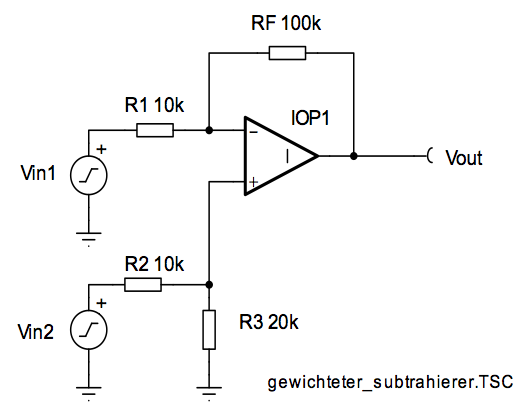
\includegraphics[width=6cm]{./bilder/gewichtsub.png}
            \end{minipage}\\
\newpage


		\subsubsection{Mehrfach-Addierer-Subtrahierer \formelbuch{3-23}} 		
		\begin{minipage}[b]{12cm}
		1. Man waehlt $R_{F}$\\
		2. Man waehlt $R_{P}$, wobei oft $R_{P}=R_{F}$ gesetzt wird. (optional)\\
		3. $R_{n}=\frac{R_{F}}{\left|A_{n}\right|}$ oder
			$R_{n}=\frac{R_{P}}{\left|A_{n}\right|}$\\ 
		4. Verstärkungsbedingung: $A_{N1} +
		\ldots + A_{Nn} = A_{P1} + \ldots + A_{Pn}$ \\Falls unerfüllt, muss ein Dummyeingang hinzugefügt werden!
		\end{minipage}
		\begin{minipage}{6cm}
          	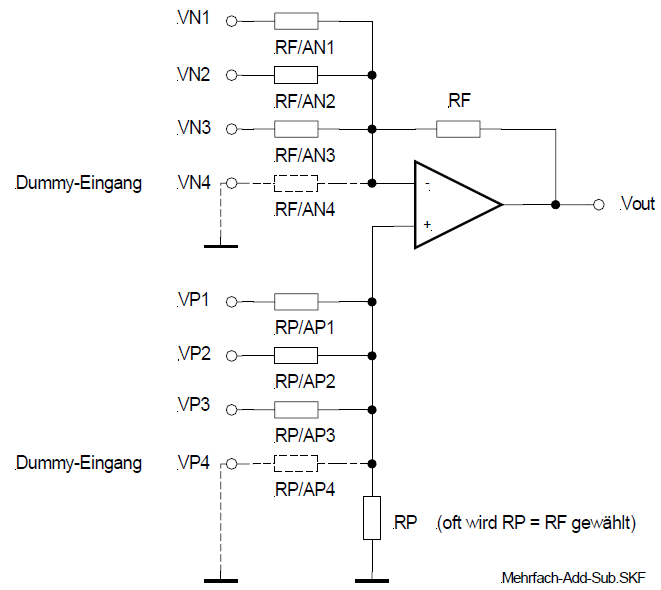
\includegraphics[width=6cm]{./bilder/mehrfach-addierer-subtrahierer.png} 
        \end{minipage}\\
		
		
\hrule

		\subsubsection{Instrumentenverstärker \formelbuch{3-25}}
		\begin{minipage}[b]{12cm}
		\hspace*{10mm}\fbox{$A_{diff}=\frac{V_{out}}{V_{diff}}=\frac{V_{P}-V_{N}}{V_{inP}-V_{inN}}
		=\frac{2R_{1}+P}{P}=\frac{2R_{1}}{P}+1$}\\
		\end{minipage}
		\begin{minipage}{6cm}
          	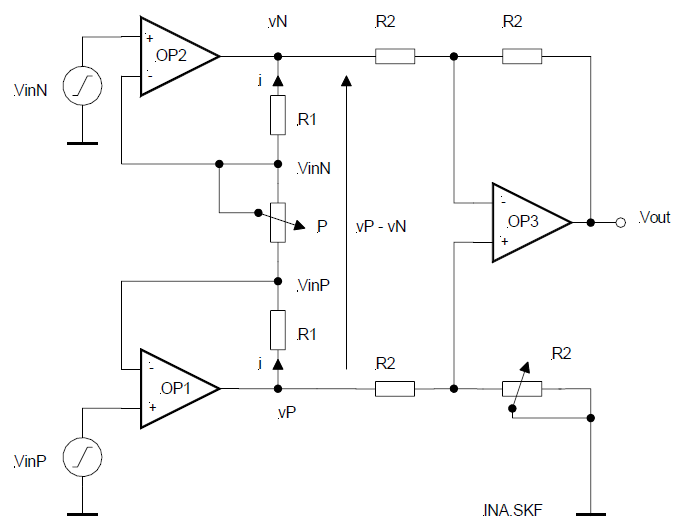
\includegraphics[width=6cm]{./bilder/Instrumentationsverstaerker.png} 
        \end{minipage}\\
		
\hrule

		\subsubsection{Differenzverstärker \formelbuch{3-21}}
			\begin{minipage}[b]{12cm}
            	\hspace*{10mm}\fbox{$A_{diff}=\frac{v_{out}}{(v_{in2}-v_{in1})}$}\\
            	\\ Widerstandsbedingung für den Differenzverstärker\\ \\
            	\hspace*{10mm}\fbox{$\frac{R_F}{R_1}=\frac{R_3}{R_2}$}
            	\hspace{15mm}\fbox{$A_{diff}=\frac{R_F}{R_1}=\frac{R_3}{R_2}$}
            	\hfill
            \end{minipage}
			\begin{minipage}{6cm}
            	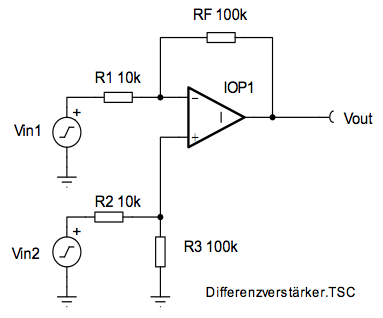
\includegraphics[width=6cm]{./bilder/differenzver.png}
            \end{minipage}\\

\newpage

		\subsubsection{Komparatorschaltung \formelbuch{3-27}}
			\begin{minipage}{18cm}
            	Wenn ein Operationsverstärker als {\it Verstärker ohne
            	Gegenkopplung} betrieben wird, spricht man von einer {\it
            	Komparatorschaltung}. Der Operationsverstärker wird dann als {\it
            	Komparator} betrieben.\\
            	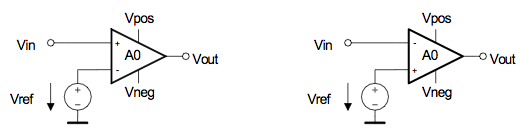
\includegraphics[width=16cm]{./bilder/komparator.png}\\
            	Beim nichtinvertierenden Komparator (links)\\
            	\hspace*{10mm}\fbox{$V_{out}=V_{out\hspace{1mm}max}=V_{pos}-V_{Rand}
            	\mbox{ wenn } V_{in} > V_{ref}\pm V_{OS} \mbox{ bzw. } 
            	V_{diff}\pm V_{OS}>0$}\\
            	\hspace*{10mm}\fbox{$V_{out}=V_{out\hspace{1mm}min}=V_{neg}+V_{Rand}
            	\mbox{ wenn } V_{in} < V_{ref}\pm V_{OS} \mbox{ bzw. } 
            	V_{diff}\pm V_{OS}<0$}\\ \\
            	Beim invertierenden Komparator (rechts)\\
            	\hspace*{10mm}\fbox{$V_{out}=V_{out\hspace{1mm}max}=V_{pos}-V_{Rand}
            	\mbox{ wenn } V_{in} < V_{ref}\pm V_{OS} \mbox{ bzw. } 
            	V_{diff}\pm V_{OS}<0$}\\
            	\hspace*{10mm}\fbox{$V_{out}=V_{out\hspace{1mm}min}=V_{neg}+V_{Rand}
            	\mbox{ wenn } V_{in} > V_{ref}\pm V_{OS} \mbox{ bzw. } 
            	V_{diff}\pm V_{OS}>0$}\\
            \end{minipage}

\hrule
		
		\subsubsection{Schmitt-Trigger \formelbuch{3-31}}
		Nichtinvertierender Schmitt-Trigger\\
			\begin{minipage}{9cm}
	          	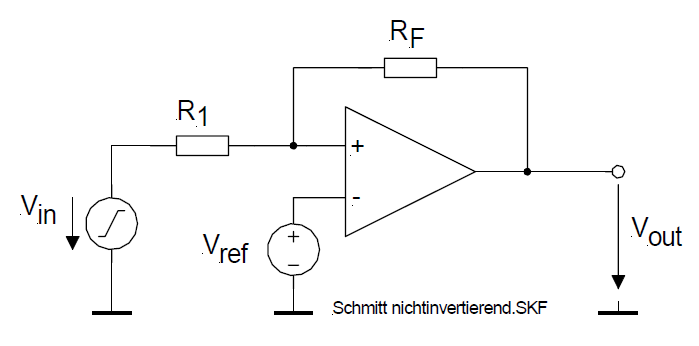
\includegraphics[width=8cm]{./bilder/n-schmitt.png} 
	        \end{minipage}
			\begin{minipage}{9cm}
	          	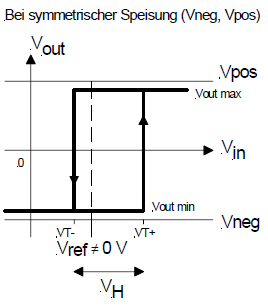
\includegraphics[width=4cm]{./bilder/n-schmitt-kennlinie.png} 
	        \end{minipage}\\
		Invertierender Schmitt-Trigger\\
			\begin{minipage}{9cm}
	          	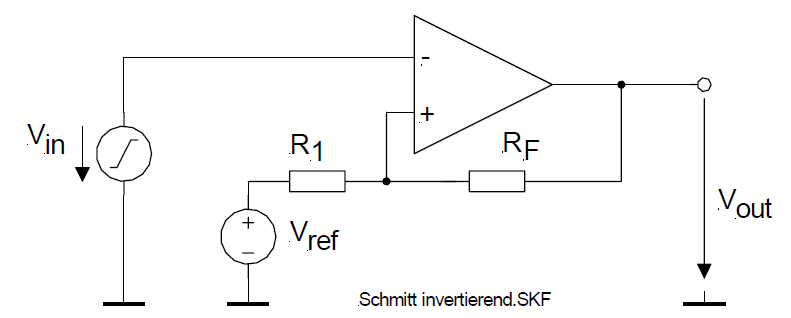
\includegraphics[width=8cm]{./bilder/i-schmitt.png} 
	        \end{minipage}
			\begin{minipage}{9cm}
	          	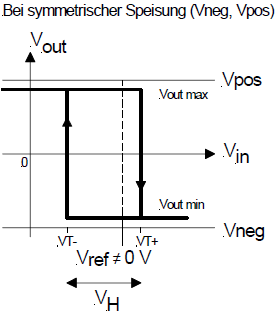
\includegraphics[width=4cm]{./bilder/i-schmitt-kennlinie.png} 
	        \end{minipage}\\
			
			\begin{minipage}{18cm}
               	Hysteresespannung:\\
               	\hspace*{10mm}
               	\begin{tabular}{| c | c |}
                \hline
                Nichtinvertierender Schmitt-Trigger & Invertierender
                Schmitt-Trigger\\
                \hline
                $V_H=(V_{out \hspace{1mm} max}-V_{out \hspace{1mm}
                min})\frac{R_1}{R_F}$ &
                $V_H=(V_{out \hspace{1mm} max}-V_{out \hspace{1mm}
                min})\frac{R_1}{R_1+R_F}$\\
                \hline
            \end{tabular}\\ \\
				Schwellspannung:\\
				\hspace*{10mm}
			\begin{tabular}{| c | c |}
                \hline
                Nichtinvertierender Schmitt-Trigger & Invertierender
                Schmitt-Trigger\\
                \hline
                $V_{T+}=V_{ref}+(V_{ref}-V_{out
                \hspace{1mm} min})\frac{R_1}{R_F}$ &
                $V_{T+}=V_{ref}+(V_{out \hspace{1mm}
                max}-V_{ref})\frac{R_1}{R_1+R_F}$\\
                \hline
                $V_{T-}=V_{ref}-(V_{out
                \hspace{1mm} max}-V_{ref})\frac{R_1}{R_F}$ &
                $V_{T-}=V_{ref}-(V_{ref}-V_{out \hspace{1mm}
                min})\frac{R_1}{R_1+R_F}$\\
                \hline
            \end{tabular}\\
            \end{minipage}

\newpage
	
		\subsubsection{Differentiator \formelbuch{3-42}}
			\begin{minipage}[b]{12cm}
           		Beim Differentiator gilt $v_{out}=v_N-i_1 \cdot R_F$ wobei
           		$v_N=0$\\ \hspace*{10mm}\fbox{$i_1=C_1 \cdot \frac{dv_C}{dt}$}\\
           		\hspace*{10mm}\fbox{$v_{out}=-R_FC_1 \frac{dv_{in}}{dt}$}\\
           		Die Elemente $C_F$ und $R_1$ sind optional. \\
           		Sie beheben jedoch Probleme die ohne \\
           		sie entstehen (siehe elemenarer Differentieator). \\
           		Mit $C_F$ und $R_1$: \\
           		- Keine differentiation bei hoeheren Frequenzen. \\
           		- Limitierte Verstaerkuing bei hoeheren Frequenzen. \\
           		- Eingangswiderstand immer groesser $R_1$ \\ 
           		$\rightarrow$ keine Belastung der Signalquelle
           
           	\end{minipage}
			\begin{minipage}{6cm}
           		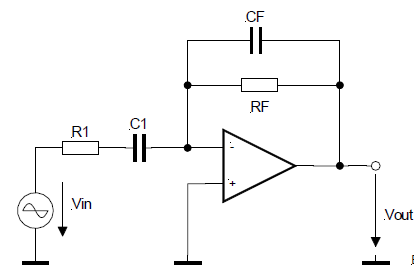
\includegraphics[width=6cm]{./bilder/differentiator.png}
           	\end{minipage}

\hrule

		\subsubsection{Integrator \formelbuch{3-45}} 
		\vspace{1cm}
		\begin{minipage}[b]{12cm}
		\hspace{8mm} \fbox{$v_{out}=-\frac{1}{RC} \int{v_{in}}dt +
		v_{out\hspace{1mm}Anfang} $}\\
		\hspace{8mm} \fbox{$\frac{dv_{out}}{dt}=-\frac{v_{in}}{RC}$}\\
		\end{minipage} 
		\begin{minipage}{6cm}
          	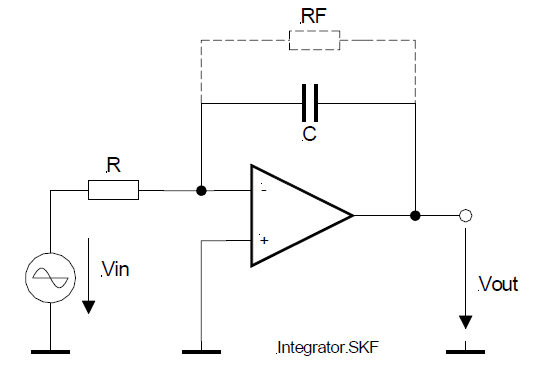
\includegraphics[width=6cm]{./bilder/integrator.png} 
        \end{minipage}\\
		
\hrule
		\subsection{Fehlereinflüsse des Opamp \formelbuch{3-51}}
		\subsubsection{Verstärkungsfehler bei endlicher Closed-Loop-Verstärkung
		\formelbuch{3-51}}
			\begin{minipage}{12cm}
               	beim nichtinvertierenden Verstärker 
               	\fbox{$A_{CL \hspace{1mm} ideal}=\frac{R_F}{R_1}+1$}\\
               	beim invertierenden Verstärker
               	\hspace{8mm}\fbox{$A_{CL \hspace{1mm}
               	ideal}=-\frac{R_F}{R_1}$}\\ \\
               	Beim invertierenden Verstärker ist eine kleine Korrektur
               	anzubringen: 
               	\hspace*{10mm}\fbox{$\frac{1}{A_{CL \hspace{1mm}
               	real}}=\frac{1}{A_{CL \hspace{1mm} real}}+\frac{1}{nA_{OL}}$}\\
	        \end{minipage}
			\begin{minipage}{6cm}
               	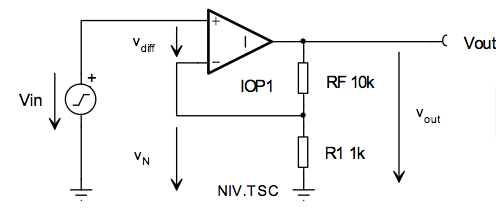
\includegraphics[width=6cm]{./bilder/verstaerkungsfaktor.png}
            \end{minipage}

\hrule

		\subsubsection{Common-Mode-Fehler \formelbuch{3-60}}
			\begin{minipage}{6cm}
            	Mittelspannung: \fbox{$V_M=\frac{V_{pos}+V_{neg}}{2}$}\\
            	Offsetspannung: \fbox{$V_{OS}=\frac{V_{CM}}{CMRR_{lin}}$}
            \end{minipage}
			\begin{minipage}{12cm}
            	Opamp-Eingangsspannung: \fbox{$V_{OP \hspace{1mm} IN}=\frac{V_P+V_N}{2}$}\\
            	Ausgangs-Fehlerspannung: \hspace{0.2mm}
            	\fbox{$V_{out \hspace{1mm} E}=\left|V_{OS}\right| \cdot A_{CL+}=\left| \frac{\Delta V_{CM}}{CMRR_{lin}}\right|A_{CL+}$}
            \end{minipage}

			\begin{minipage}{18cm}
            	Common-Mode-Spannung:
            	\fbox{$V_{CM}=V_{OP \hspace{1mm} IN}-V_M=V_P- \frac{V_{pos}+V_{neg}}{2} \mbox{ bzw. }V_N- \frac{V_{pos}+V_{neg}}{2}$}\\
            	\hspace*{4.2cm}\fbox{$V_{CM}\frac{V_{P}+V_{N}}{2}-V_M$}\\
            	Lineare Definition: \hspace{11mm}
            	\fbox{$CMRR_{lin}=\frac{dV_{CM}}{dV_{OS}}=10^{\frac{CMRR_{dB}}{20}}$}
            	\hspace{11mm}
            	\fbox{$CMRR_{lin}=\frac{A_{OL}}{A_{CM}}$}\\
            	Logarithmische Definition:
            	\fbox{$CMRR_{dB}=20 \cdot log(CMRR_{lin})=20 \cdot log\frac{dV_{CM}}{dV_{OS}}$}\\
            \end{minipage}

\newpage
		
		\subsubsection{Offsetspannungsfehler \formelbuch{3-53}}
			\begin{minipage}{18cm}
            	Im Closed-Loop-Betrieb ist die Ausgangs-Fehlerspannung:\hspace{6mm}
            	\fbox{$V_{out \hspace{1mm}E}=V_{OS}\left( 1+\frac{R_F}{R_1}
            	\right)$} allgemein: $V_{out \hspace{1mm}E}=V_{OS}
            	\cdot {A_{CL}}^{+}$\\
            	Im Open-Loop-Betrieb ist die Ausgangs-Fehlerspannung:\hspace{6mm}
            	\fbox{$V_{out \hspace{1mm}E}=V_{OS}
            	\cdot {A_{CL}}^{+}$}\\
            \end{minipage}

\hrule
		
		\subsubsection{Eingangsstromfehler \formelbuch{3-54}}
			\begin{minipage}{18cm}
              Wenn die Opamp-Eingangsströme gleich gross sind
              ($I_{N}=I_{P}$) und die Gleichstromwiderstände,
              die von jedem Opamp-Eingang nach Masse führen, 
              ebenfalls gleich gross gewählt werden, heben sich die
              Ausgangsspannungsfehler, die durch $I_{N}$ und $I_{P}$
              erzeugt werden, gegenseitig auf. \\
              Allgemeine Formel für den
              Eingangsstromfehler:
                \hspace{20mm}
                \fbox{$V_{out \hspace{1mm}E}=I_N R_F-R_2 I_P\left( 1+\frac{R_F}{R_1} \right)$}\\ Widerstandsbedingung für Eingangsstromkompensation: \hspace{7.5mm}
            	\fbox{$R_2=\frac{R_F R_1}{R_F+R_1}=R_F // R_1$}\\
            \end{minipage}\\
			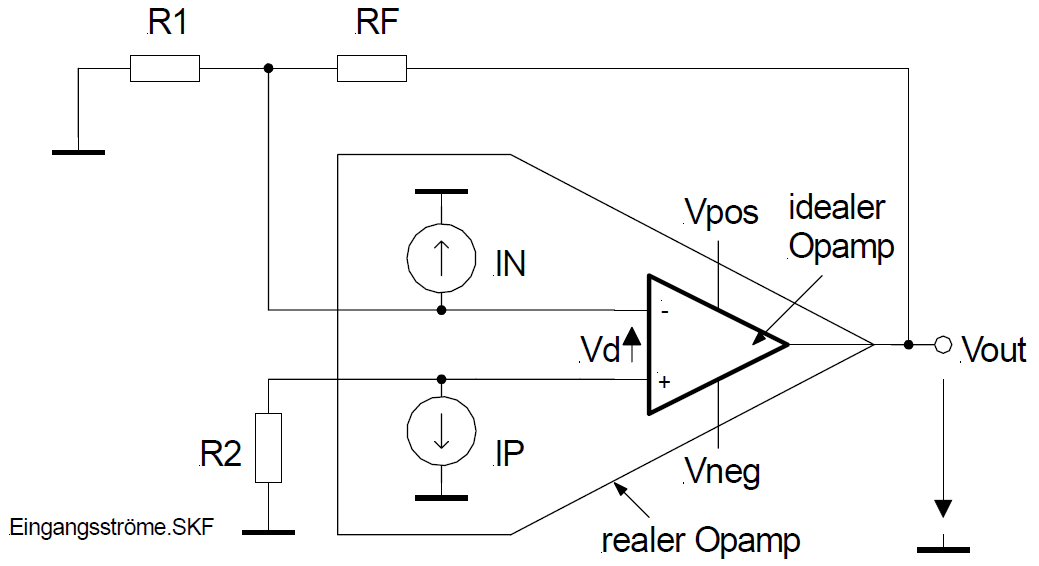
\includegraphics[width=8cm]{./bilder/eingangsstromfehler.png}


\hrule

		\subsubsection{Eingangsstromkompensation ohne AC-Zweige \formelbuch{3-54}}
			\begin{minipage}[b]{6cm}
            	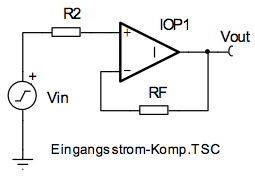
\includegraphics[height=3cm]{./bilder/spannungsfolger.png}\\
            	\centerline{{\bf Spannungsfolger}}\\ \\
            	$R_2$ sei ein gegebener Quellen-Widerstand\\
            	{\bf $R_F$ muss eingefügt werden}\\ \\
            	\fbox{$R_F=R_2$}
            \end{minipage}\hfill
			\begin{minipage}[b]{6cm}
            	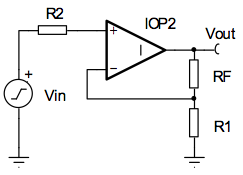
\includegraphics[height=3cm]{./bilder/nichtinver}\\
            	\centerline{{\bf Nichtinvertierender Verstärker}}\\ \\
            	Hier sei der Quellenwiderstand
            	vernachlässigbar.\\ {\bf $R_2$ muss eingefügt werden}\\ \\
            	\fbox{$R_2=R_F//R_1$}
            \end{minipage}\hfill
			\begin{minipage}[b]{6cm}
            	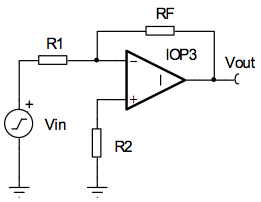
\includegraphics[height=3cm]{./bilder/inver}\\
            	\centerline{{\bf Invertierender Verstärker}}\\ \\ \\ \\
            	{\bf $R_2$ muss eingefügt werden}\\ \\
            	\fbox{$R_2=R_F//R_1$}
            \end{minipage}
			\begin{minipage}{18cm}
            	\vspace{3mm}
				\textbf{Ausgangsspannungsfehler} auf Grund des \textbf{Offsetstromes} (nur bei
				Kompensation(!)):
				\fbox{$V_{out \hspace{1mm}E}=\left|I_{OS}\right| \cdot R_F$}\\
			\end{minipage}
\hrule

		\subsubsection{Power-Supply-Fehler \formelbuch{3-58}}
			\begin{minipage}{18cm}
            Die grösse $PSRR$ (Power Supply Rejection Ratio, Speisespannungsunterdrückung)\\
            Offsetspannung: \fbox{$V_{OS}=\frac{\Delta V_{Supply}}{PSRR_{lin}}$}
            \hspace{10mm}
            Ausgangsspannungsfehler:
            \fbox{$V_{out \hspace{1mm}E}=\left|V_{OS}\right| A_{CL+}=\left| \frac{\Delta V_{Supply}}{PSRR_{lin}}\right| A_{CL+}$}\\
            Lineare Definition: \hspace{11mm}
            \fbox{$PSRR_{lin}=\frac{dV_{Supply}}{dV_{OS}}=10^{\frac{PSRR_{dB}}{20}}$}\\
            Logarithmische Definition:
            \fbox{$PSRR_{dB}=20 log PSRR_{lin}=20 log \frac{dV_{Supply}}{dV_{OS}}$}\\
            \end{minipage}

\hrule

		\subsubsection{Zusammenfassung aller Fehlereinflüsse \formelbuch{3-63}}
			\begin{minipage}{18cm}
            	\fbox{$V_{out\hspace{1mm}E\hspace{1mm}total}=A_{CL+}\cdot\left[\left|V_{OS}\right|+\frac{\left|V_{CM}\right|}{CMRR}
            	+\frac{\left|\Delta V_{Supply}\right|}{PSRR}\right]+\left|I_{OS}\right|R_F$}\\
            \end{minipage}

\newpage

		\subsection{Dynamische Eigenschaften des Opamp \formelbuch{3-66}}
			\begin{minipage}{18cm}
            	dB-Verstärkung: \hspace{4.5mm}
            	\fbox{$A_{dB}=20 \cdot log A_{lin}$}\\
            	lineare Verstärkung:
            	\fbox{$A_{lin}=10^{\frac{A_{dB}}{20}}$}\\ \\
            	Verstärkungs-Bandbreite-Produkt GBP (Gain-Bandwidth-Product)\\
            	Bandbreite des gegengekoppelten {\it nichtinvertierenden} Verstärkers:
            	\fbox{$f_{CL+}=\frac{GBP}{A_{CL \hspace{1mm}lin}}$}\\
            	Bandbreite des gegengekoppelten {\it invertierenden} Verstärkers: \hspace{6.5mm}
            	\fbox{$f_{CL}=\frac{GBP}{\left| A_{CL \hspace{1mm}lin}\right|+1}$}\\ \\
            	{\bf Gesetz vom Konstanten Verstärkungs-Bandbreite-Produkt:} \\ \\
            	Für jeden Punkt auf der mit -20dB abfallenden Frequenzgang-Gerade ist das
            	Produkt aus Verstärkung und zugehöriger Frequenz konstant gleich GBP, d.h. $A_{lin}\cdot f=GBP=konst$\\
            \end{minipage}
		\subsubsection{Slew-Rate}
		min. SR bei einem Sprungsignal \hspace{4mm}
		\fbox{$SR\geq\frac{0.8V_{step}}{t_{anstieg}}$}\\ 
		min. SR bei einem Sinussignal \hspace{4.5mm} 
		\fbox{$SR\geq V_{amplitude}\omega=V_{amplitude}2\pi f$}\\
		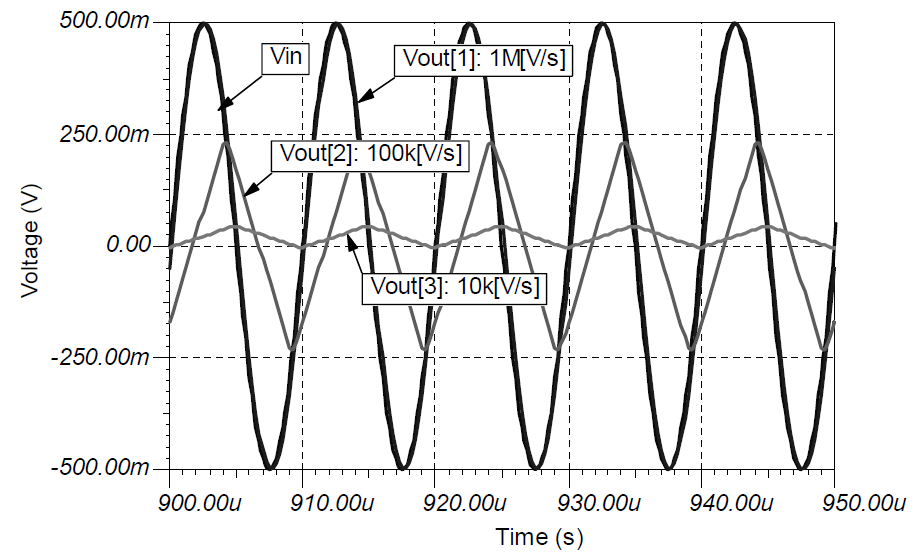
\includegraphics[height=5cm]{./bilder/slew-rate.png}\\

\newpage

	\section{Kühlung von Bauteilen \formelbuch{4}}
	
	\subsection{Thermisches Schema \formelbuch{4-6}}
		Generell gilt im thermischen (elektrischen) Schema: 
		\begin{itemize}
	      \item Jeder Knoten besitzt eine Temperatur gegen die Umgebung (el. Spannung gegen Masse).
	      \item In jedem Zweig fliesst eine thermische Leistung (el. Strom).
	      \item Zwischen den Knoten liegen thermische Widerstände (el. Widerstände).
    \end{itemize}   
    
		\begin{center}
	  		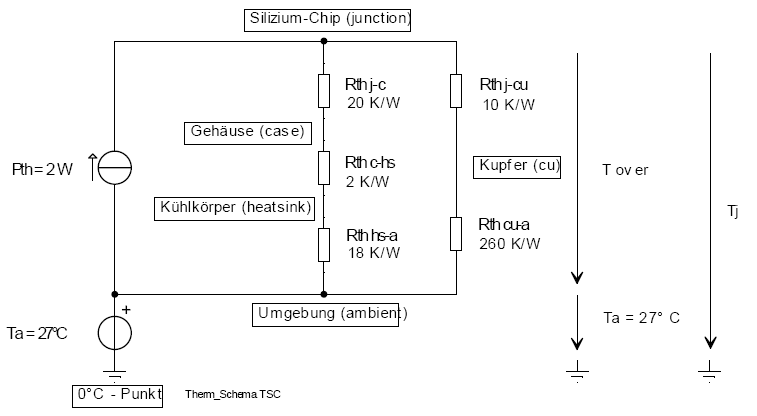
\includegraphics[height=6cm]{../Elo1/bilder/thermisches_schema2.png} \\
	  	\end{center}

		\begin{center}
	  		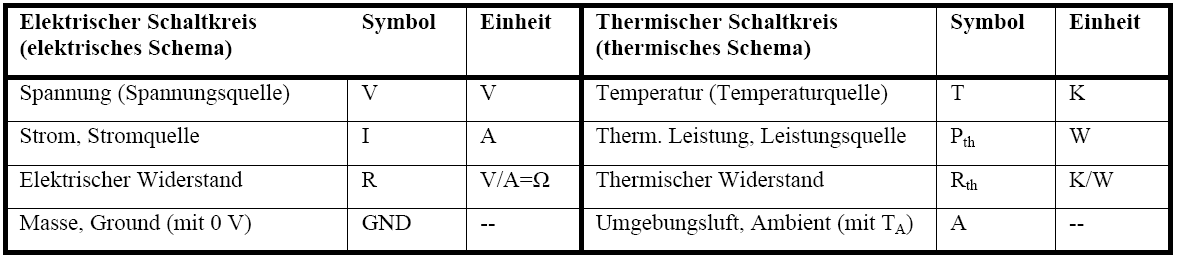
\includegraphics[height=3.5cm]{../Elo1/bilder/thermisches_schema.png} \\
	  	\end{center} 
    
		\begin{center}
	  		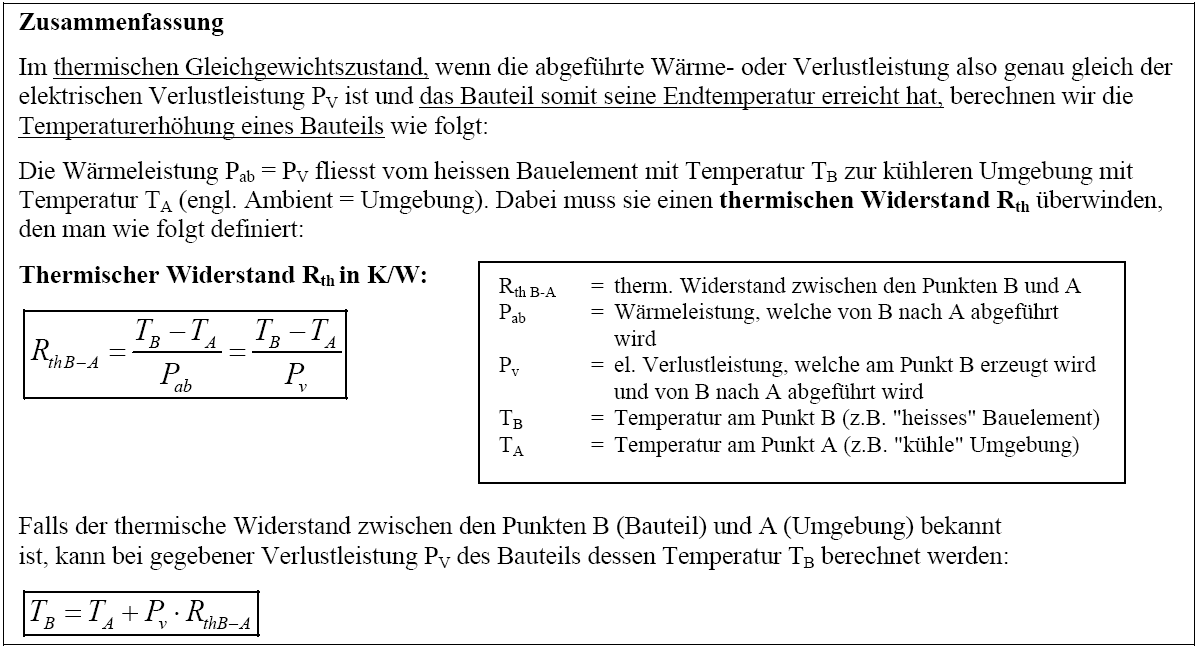
\includegraphics[width=16cm]{../Elo1/bilder/thermisches_schema3.png}
	  	\end{center}


\end{document}
